\documentclass[12pt]{article}
\usepackage{graphicx}
\usepackage {color}
\usepackage{pdfpages}
\usepackage{float}
\usepackage{changebar}
\usepackage{enumitem,amssymb}
\renewcommand{\familydefault}{\sfdefault}
\usepackage[margin=1.2in]{geometry}
\usepackage{graphicx}
\usepackage{wrapfig}
\usepackage[super]{cite}
\usepackage{subcaption}
\usepackage[table]{xcolor}
\usepackage{amsmath}
\usepackage[sort, numbers]{natbib}
\usepackage{multirow}
\usepackage{tabularx}
\usepackage{siunitx}



%%%%%%%%%%%%Defining the margins %%%%%%%%%%%%%%%%%%%%%
\textheight 9.in
\textwidth 6.5in
\topmargin -.5in
\oddsidemargin 0in
\setlength{\parskip}{\smallskipamount}

%%%%%%%%%%%%%%Specific Commands %%%%%%%%%%%%%%%%%%
\newcommand{\eg}{{\em e.g.,}}
\newcommand{\ie}{{\em i.e.,}}
\newcommand{\etc}{{\em etc.,}}
\newcommand{\etal}{{\em et al.}}
\newcommand{\degrees}{{$^{\circ}$}}
\newcommand{\fig}[1]{\textbf{Figure #1}}
\DeclareMathOperator*{\argmin}{argmin}
\DeclareMathOperator*{\argmax}{argmax}
\DeclareMathOperator*{\diver}{div}
%%%%%%%%%%%%%%%%%%%%%%%%%%%% Setting to control figure placement
% These determine the rules used to place floating objects like figures 
% They are only guides, but read the manual to see the effect of each.
\renewcommand{\topfraction}{.9}
\renewcommand{\bottomfraction}{.9}
\renewcommand{\textfraction}{.1}
\renewcommand{\familydefault}{\sfdefault} %setting the san serif font

%%%%%%%%%%%%%%%%%%%%%%%% Line spacing
% Use the following command for ``double'' spacing
%\setlength{\baselineskip}{1.2\baselineskip}
% and this one for an acceptable NIH spacing of 6lpi based on 11pt
%\setlength{\baselineskip}{.9\baselineskip}
% The baselineskip does not appear to work when we include a maketitle
% command in the main file.  Something there must set the line spacing
% If we use this next command, then things seem to work.
\renewcommand{\baselinestretch}{.9}

\setcounter{secnumdepth}{0} %make no numbers but have a table of contents


\begin{document}

\title{TV vs H1 Inpainting}
\author{Jake Bergquist, u6010393 }
\maketitle

\section{Introduction}
\par{}
For this midterm project we were tasked swith formulating and implementing H1 and total variation in painting methods to replace corrupted data from images. In the case of the H1 inpainting we do so by implementing a H1 denoising alogrithm  which, in short, performs an iterative laplacian blur into the missing area. If we consider the H1 denoising formulation (Equation~\ref{EQ:H1Denoise}) we see that this function aims to estimate the denoised image, $\hat{I}~(x)$ by minimizing the difference between the sampled image ($d(x)$) and the denoised image ($I(x)$) as well as the gradient of the denoised image. By integrating these terms we find that we can simplify to Equation~\ref{EQ:H1_2} wherein our minimization changes to minimizing the sum of the inner products of $d(x)-I(x)$ with itself plus the inner product of the negative laplacin of $I(x)$ with $I(x)$. From here we get Equation~\ref{EQ:H1_3} which allows us to solve for the ideal $I(x)$ by setting it equal to zero. By using a finite difference model we can approximate the inverse of the laplacian needed to calculate for this ideal $I(x)$. Now if we consider our in painting problem instead we also want to impose the condition that we have data missing. The same denoising algorithm can be used to fill in this missing space. The entire H1 denoising algorithm boils down to applying a laplacian blur to the image. If we apply this blur into the areas where data is missing (set the corrupt data to 0) this will begin to interpolate the missing data based on the neighboring data. We can iterativly blur into the missing region while replacing the non missing data with the original measured data. This prevents the image from being overly smoothed. Finally we can perform a final H1 denoise to smooth any noise if desired.

\begin{equation}
\hat{I}(x) = \argmin_{I(x)} \frac{1}{2\sigma^2} \int_{}^{}||d(x) - I(x)||^2 dx + \frac{1}{2\alpha^2}\int_{}^{}||\nabla I(x)||^2 dx 
\label{EQ:H1Denoise}
\end{equation}

\begin{equation}
\hat{I}(x) = \argmin_{I(x)} \frac{1}{2\sigma^2}<d(x)-I(x),d(x)-I(x)> + \frac{1}{2\alpha^2}<-\Delta~I(x),I(x)>
\label{EQ:H1_2}
\end{equation}

\begin{equation}
-\Delta~I(x) + \frac{(I(x)-d(x))}{\sigma^2} = 0
\label{EQ:H1_3}
\end{equation}

\par{}
In the case of TV denoising and inpainting we must consider the slightly different primary formulation Equation~\ref{TV:Primal}. Notice that the second term is no longer the L2 norm but the L1 norm. Thus we can no longer solve this minimization as simply as we cannot operate in Hilbert space. Thus we must use a dual space formulation for this optimization. Because of the relationship outlined in equation~\ref{TV:L1toDiv} we can rewrite Equation~\ref{TV:Primal} as Equation~\ref{TV:preDual}. By differentiating this equation and setting equal to zero we get the dual formulation of our problem in Equation~\ref{TV:dual}. By substituting \ref{TV:dual} into \ref{TV:Primal} and completing the square by adding a constant term $d^2(x)dx$ we get a more simple primal formulation in Equation~\ref{TV:simplePrimal}. All of this defines TV denoising, whicl allows for the preservation of discontinuous edges via the L1 term in the primal form which is not possible in the smoothing done by the L2 term of the H1 denoising. To optimize the TV probelm we can either take steps in the primal and dual directions by optimizing over \ref{TV:Primal} and \ref{TV:dual} or we can optimize over the full dual using \ref{TV:simplePrimal}. However, to modify this formulation to account for an image with missing data we have two options. In both we impose a $m(x)$ mask term that is zero where we are missing data and 1 where we are not missing data. By multiplying this mask pointwise across the first term in \ref{TV:Primal} we account for the fact that there is no contributing data at those locations. However this changes our formulation of \ref{TV:simplePrimal} significantly. Because we now have zeros in $d(x)$ we can no longer formulate \ref{TV:simplePrimal} as this would result in division by zero. We can either perform this optimization of inpainting by using the primal dual formulation (\ref{TV:Primal} and \ref{TV:dual}) (again like in H1, using the interpolation into th emissing region, then at each iteration replacing the area outside of the missing data area with the original measured image) or we can attempt to formulate the full dual problem like in \ref{TV:simplePrimal}. In this report I will present results from the former of these, but I will present a formulation for the second. Due to some error along the way I was unable to get the full dual formulation to function.
\begin{equation}
\hat{I}(x) = \argmin_{I(x)} \frac{1}{2\sigma^2} \int_{}^{}||d(x) - I(x)||^2 dx + \frac{1}{alpha^2}\int_{}^{}||\nabla I(x)|| dx 
\label{TV:Primal}
\end{equation}
\begin{equation}
||\nabla~I(x)|| = \sqrt{I_x^2(x)+I_y^2(x)} = \argmax_{||w(x)||<1}-I(x)\diver(w(x))
\label{TV:L1toDiv}
\end{equation}

\begin{equation}
\hat{I}(x) =\argmax_{||w(x)||<1} \argmin_{I(x)} \frac{1}{2\sigma^2} \int_{}^{}||d(x) - I(x)||^2 dx - \frac{1}{2\alpha^2}\int_{}^{}I(x)\diver(w(x)) dx 
\label{TV:preDual}
\end{equation}

\begin{equation}
\hat{I}(x) =\sigma^2\diver(w(x)) + \alpha^2d(x)
\label{TV:dual}
\end{equation}

\begin{equation}
\hat{I}(x) =\argmax_{||w(x)||<1} -\int_{}^{}\alpha^2\diver(w(x)) + \frac{d(x)}{\sigma^2}
\label{TV:simplePrimal}
\end{equation}

\par{}
To formulate the full dual TV inpainting we must ad a term to the primal problem that fixes our division by zero problem. This is seen in Equation~\ref{TV:inPainPrimal} where we add a $\phi$ weighted term that adds a constant $c$ which prevents a division by zero error. Taking the derivative of \ref{TV:inPainPrimal}, setting it to zero, and a bit of rearrangement gives us \ref{TVI:1}. By defining \ref{EQ:A} and \ref{EX:B} we can simplify to \ref{TVI:2} as our dual formula. Substituting \ref{TVI:2} into \ref{TV:inPainPrimal} we get a very long equation~\ref{TVI:3}. After using the fact that $m(x)^2 = m(x)$, defining \ref{EQ:C} and \ref{EX:E} we get \ref{TVI:4}. The goal at this point is to group terms that are linear in $w(x)$, and those that are quadratic in $w(x)$. By expanding \ref{TVI:4} and grouping these terms we get \ref{TVI:5} with $F(X),G(X),H(x)$ defined as shown. With this we can define our full dual step as shown in \ref{EX:W}. In practice this produces an all zeros or all ones image. Thus there is likely an error involving the multiplication of the mask.


\begin{equation}
\hat{I}(x) = \argmin_{I(x)} \frac{1}{2\sigma^2} \int_{}^{}m(x)||d(x) - I(x)||^2 dx + \alpha\int_{}^{}||\nabla I(x)|| dx + \frac{1}{2\phi^2}\int_{}^{}||I(x)-C||^2 dx
\label{TV:inPainPrimal}
\end{equation}

\begin{equation}
\hat{I}(x) =\frac{\phi^2m(x)d(x) + \sigma^2\phi^2\alpha\diver(w(x))+\sigma^2C}{\phi^2m(x)+\sigma^2}
\label{TVI:1}
\end{equation}

\begin{equation}
A(x) = \frac{\phi^2m(x)d(x) + \sigma^2C}{\phi^2m(x)+\sigma^2}
\label{EQ:A}
\end{equation}
\begin{equation}
B(x) =\frac{\sigma^2\phi^2\alpha}{\phi^2m(x)+\sigma^2}
\label{EX:B}
\end{equation}
\begin{equation}
\hat{I}(x) =A(x) + B(x)\diver(w(x))
\label{TVI:2}
\end{equation}

\begin{equation}
\begin{aligned}
\hat{I}(x) = \argmin_{I(x)} \frac{1}{2\sigma^2} \int_{}^{}||m(x)A(x) + m(x)B(x)\diver(w(x)) - m(x)d(x)||^2 dx, \\
- \alpha\int_{}^{}A(x)\diver(w(x))+B(x)\diver^2(w(x)) dx, \\
+ \frac{1}{2\phi^2}\int_{}^{}||A(X) + B(x)\diver(w(x)) - C||^2 dx
\label{TVI:3}
\end{aligned}
\end{equation}

\begin{equation}
C(x) =m(x)A(x) - m(X)d(x)
\label{EX:C}
\end{equation}
\begin{equation}
E(x) =A(x) - C
\label{EX:E}
\end{equation}

\begin{equation}
\begin{aligned}
\hat{I}(x) = \argmin_{I(x)} \frac{1}{2\sigma^2} \int_{}^{}||C(x) + m(x)B(x)\diver(w(x))||^2 dx, \\
-\alpha\int_{}^{}A(x)\diver(w(x))+B(x)\diver^2(w(x)) dx,\\
 + \frac{1}{2\phi^2}\int_{}^{}||E(X) + B(x)\diver(w(x))||^2 dx
\label{TVI:4}
\end{aligned}
\end{equation}

\begin{equation}
\hat{I}(x) = \argmin_{I(x)} \int_{}^{}F(x)\diver^2(w(x))  + \int_{}^{} G(x)\diver(w(x)) + H(x) dx
\label{TVI:5}
\end{equation}
\begin{equation}
F(x) =\frac{m(x)B(x)}{2*\sigma^2} - \alpha{}B(x) + \frac{B(x)^2}{2\phi^2}
\label{EX:F}
\end{equation}
\begin{equation}
G(x) = \frac{C(x)m(x)B(x)}{\sigma^2} - \alpha{}A(x) + \frac{E(x)B(x)}{\phi^2}
\label{EX:G}
\end{equation}
\begin{equation}
H(x) = \frac{C(x)^2}{2\sigma^2} + \frac{E(x)^2}{2\phi^2}
\label{EX:H}
\end{equation}
\begin{equation}
w(x)^{k+1} = w(x)^k + \epsilon{}(2\nabla{}(F(x)\diver(w(x)^k)) + \nabla{}G(x))
\label{EX:W}
\end{equation}

\par{}
On the other hand using the primal dual formulation is very easy. As stated before, the locations where data is missing are set to zero and the TV denoising is run. After many iterations the TV denoising will start to interpolate into the missing region. At each iteration the region outside of the missing region is returned to its starting state to prevent over filtering of the image.As I explored different alpha and sigma values I found that a sigma of 0.25 and alpha of around 500 produced good results with a small step size (0.01 for primal and dual) and a large number of iterations (1000). However I found those alpha and sigma values were not ideal for other kinds of inpaining scenarios which are shown in results. To this end I thought it would be nice to try to optimize the selection of alpha and sigma. Given that we have the uncorrupted image (a not realistic scenario) we could easily come up with a cost function to minimize within the missing data mask area as seen in \ref{EX:opt}. A few days before this assignment was due I was taught by a collaborator about how a simplex optimization algorithm works. By first taking three "random" samples of the parameter space (given that we have two parameters in this case) we can create a triangle of sampled locations. From this we can determine which of these has the maximum energy according to our Eq~\ref{EX:opt}. We can then formulate our new guess to be away from this high energy guess towards the two lower energy guesses. The two lower energy guesses and our new guess form a new triangle and the process repeats, slowly walking towards an energy minimum. This approach does potentially get stuck in local minimum but it has the advantage of not needing to calculate a gradient directly and only needs to sample as it goes. By defining the first triangle as an equilateral triangle int he space with sides equal to some step size $\epsilon$, and the new guess step such that it would make a new equilateral triangle we can easily step through the space. By slowly decreasing the new step distance we can allow the algorithm to more precisely zoom in on the minimum as it goes. Of course there are more elegant ways to implement this, but I was working with a limited time span since I learned about this (about a day and a half). I was only able to implement this for TV, but it could easily be done for H1 as well to optimize for those parameters. Additionally one could image how such an algorithm could be implemented with a different energy function that did not require the actual uncorupted image but rather used some other metric of improvement.

\begin{equation}
\argmin_{\sigma,\alpha} \sum |1-m(x)|I(x) - |1-m(x)|d(x)
\label{EX:opt}
\end{equation}

\par{}
To test these algorithms and methods, the original as well as three other corrupted images were used. Corruption two was done by removing evenly spaced vertical lines from the data. Corrupt 3 was made by randomly deleting 20\% of the image, and corrupt 4 was made by corrupting evenly spaced horizontal lines. For H1 inpainting 1000 iterations were used. For TV inpainting 40 iterations of simplex optimization were used with starting sigma at 0.01, starting alpha at 100, and optimization step at 0.01. The TV inpainting itself was done in 1000 iterations.

\section{Results}
\par{}
The resulting in painted images for H1 are shown in Figure~\ref{fig:H1} and for TV in Figure~\ref{fig:TV1}. Note how H1 performed well for corruptions 2-4, but not so well on corruption 1. Whereas TV worked well on corruption 1 but less well on 2-4. Figure~\ref{fig:TV_e} shows the energy of the TV optimization for sigma and alpha selection for each case. As can be seen all cases decrease in energy through the optimization. Notably corruption 1 has the lowest overall energy, due to the lower area of corrupted pixels. Figure~\ref{fig:TV_SA_f} and Figure~\ref{fig:TV_SA_s} show the path of the optimization of alpha and sigma selection in the different corruption cases. As can be seen there is a large difference int he overall trajectories between corruption 1 and the other corruptions.

\begin{figure}[H]
	
	
	\hspace{-1.5in}
	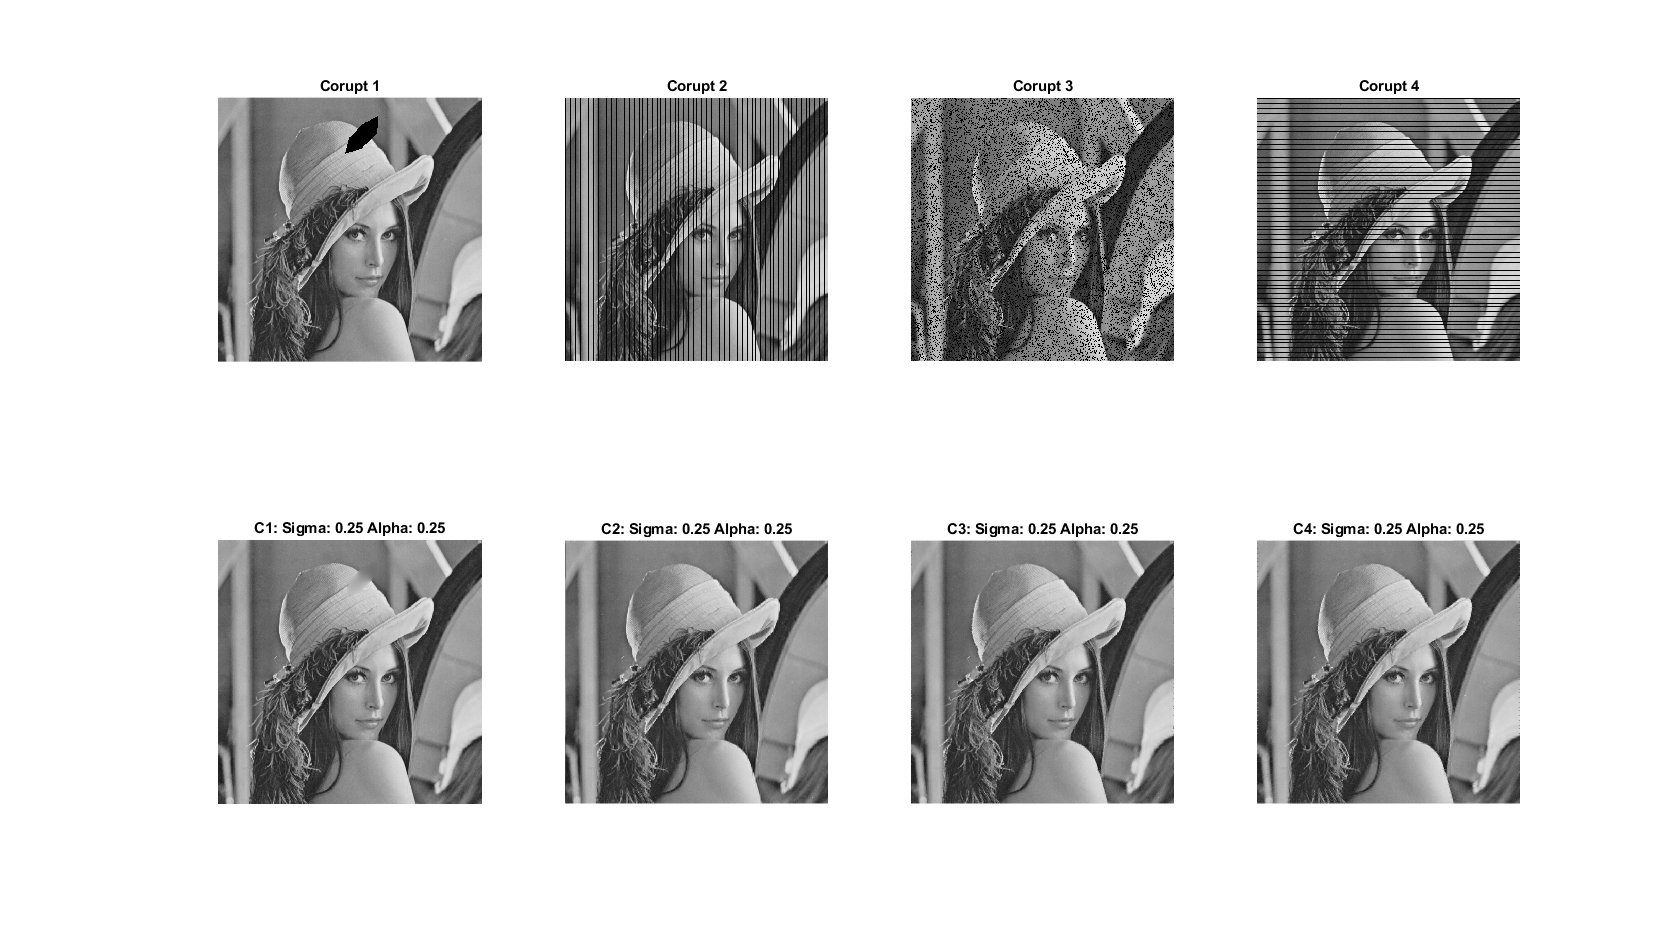
\includegraphics[width = 1.4\textwidth]{Figures/H1Results.png}
	\caption{Results from the H1 inpainting. Top row shows the corrupted images. Bottom row shows the H1 inpainted images.}
	\label{fig:H1}
\end{figure}
\begin{figure}[H]
	
	
	\hspace{-1.5in}
	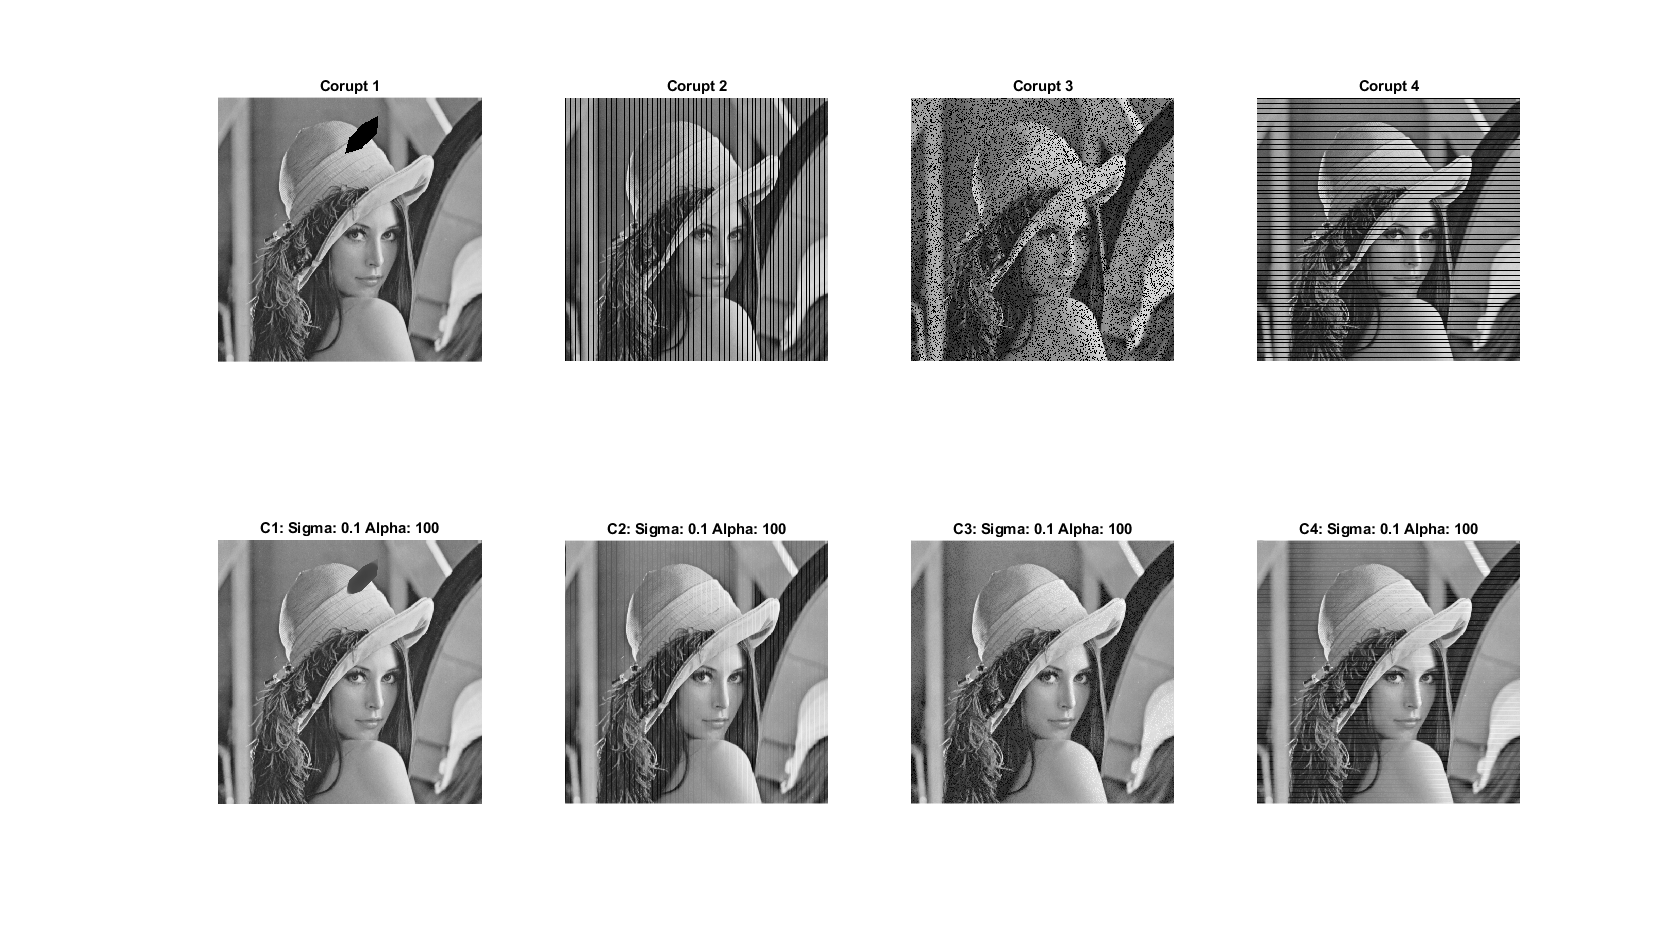
\includegraphics[width = 1.4\textwidth]{Figures/TVResults_nooptimize.png}
	\caption{Results from the TV inpainting without optimization. Top row shows the corrupted images. Bottom row shows the H1 inpainted images. Corrupt 1 in red, corrupt 2 in green, corrupt 3 in blue, corrupt 4 in pink}
	\label{fig:TV1_noopt}
\end{figure}
\begin{figure}[H]
	
	
	\hspace{-1.5in}
	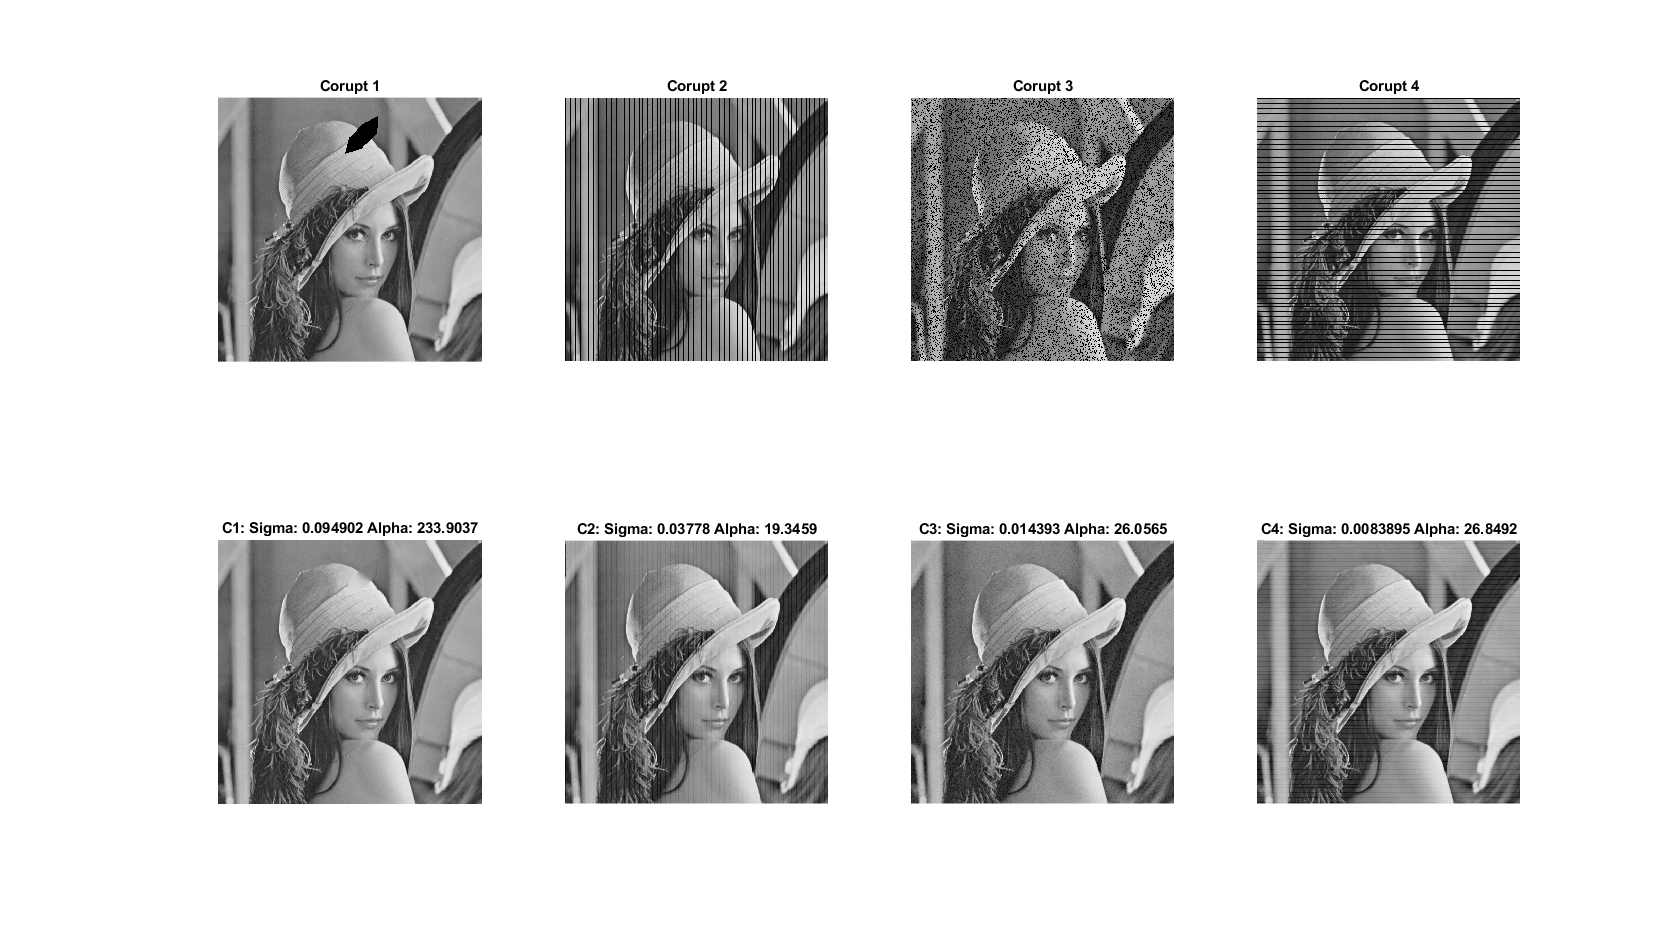
\includegraphics[width = 1.4\textwidth]{Figures/TVResults.png}
	\caption{Results from the TV inpainting with optimized sigma and alpha values. Top row shows the corrupted images. Bottom row shows the H1 inpainted images. }
	\label{fig:TV1}
\end{figure}
\begin{figure}[H]
	
	
	
	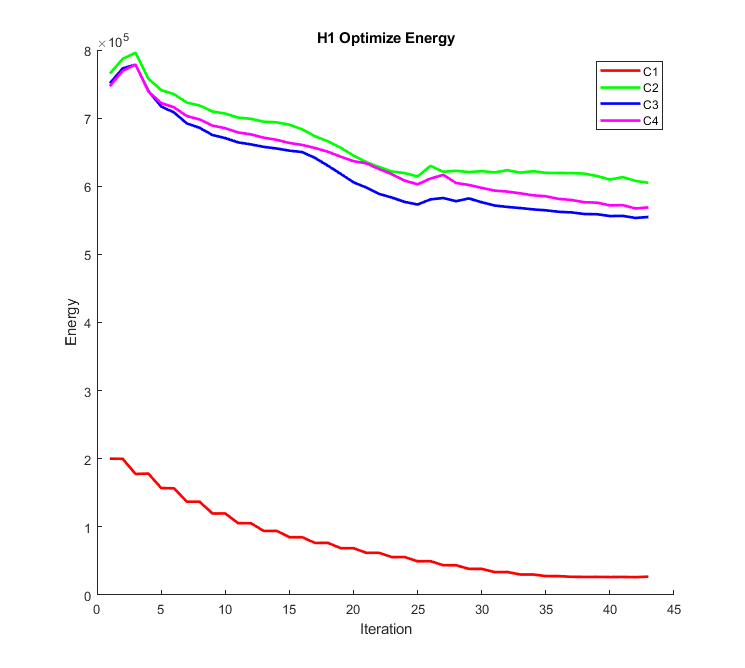
\includegraphics[width = .9\textwidth]{Figures/TVEnergy.png}
	\caption{Energy during TV sigma alpha optomization. initial sigma at 0.01, alpha at 100. Guess step size at 0.01, three initial guesses and 40 simplex steps. Corrupt 1 in red, corrupt 2 in green, corrupt 3 in blue, corrupt 4 in pink}
	\label{fig:TV_e}
\end{figure}
\begin{figure}[H]
	
	
	
	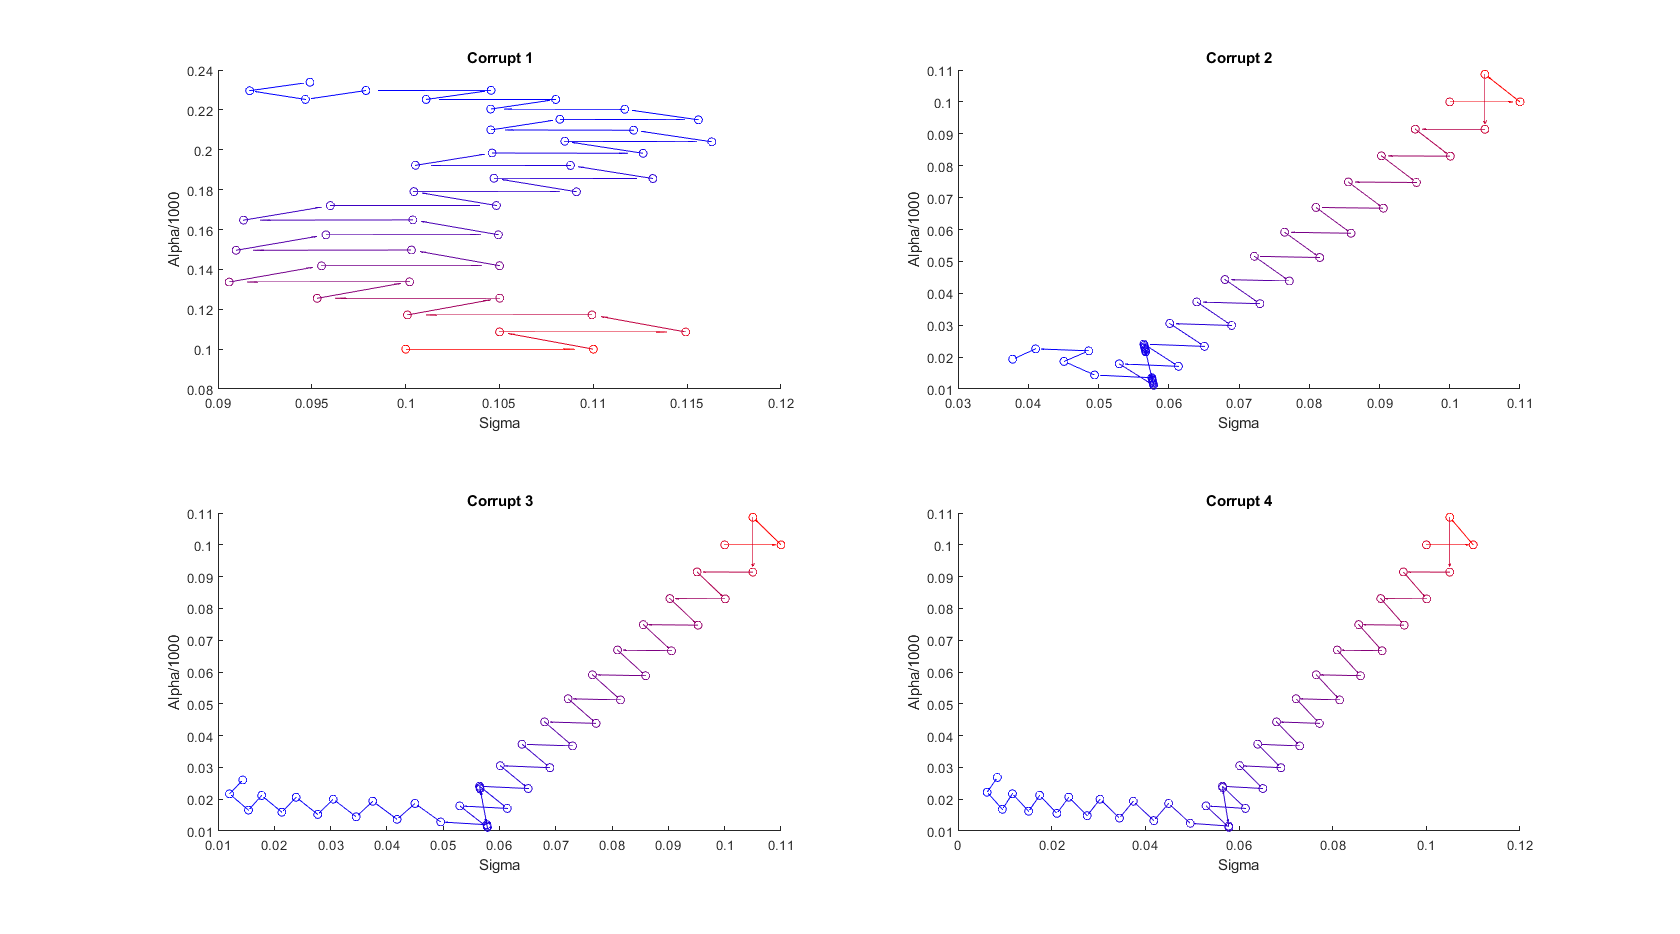
\includegraphics[width = .9\textwidth]{Figures/TVSigAlphaflat.png}
	\caption{Sigma and alpha values chosen during optimization. Higher energy guesses in red, lower energy in blue. Path of simplex steps shown by vectors.}
	\label{fig:TV_SA_f}
\end{figure}

\begin{figure}[H]
	
	
	
	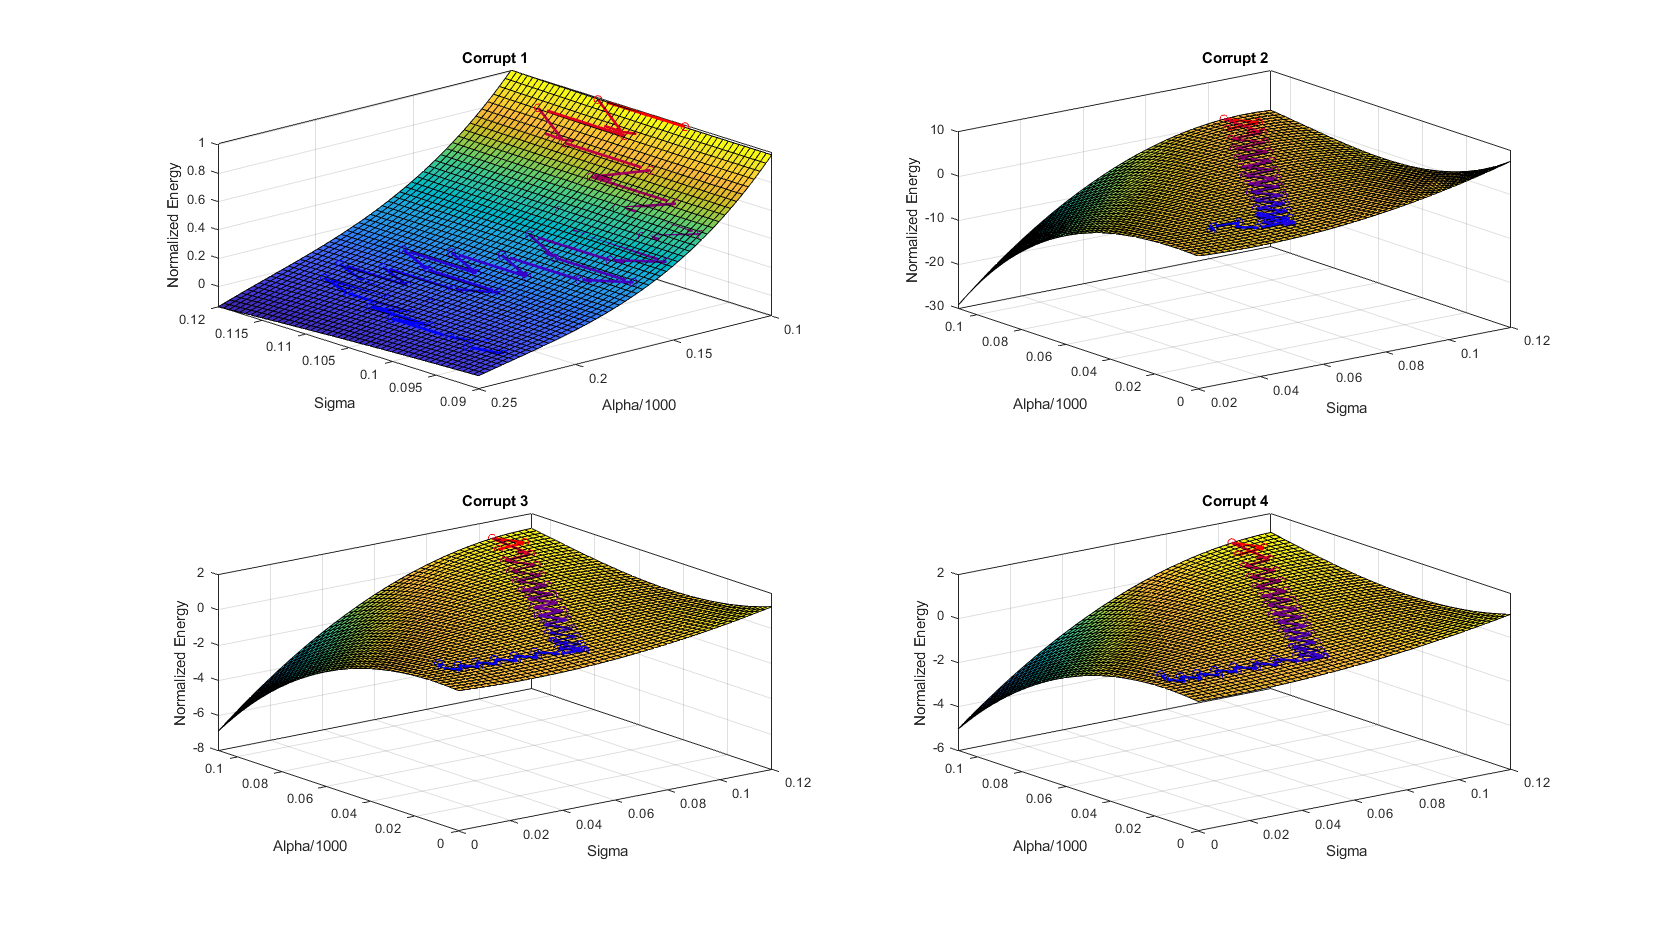
\includegraphics[width = .9\textwidth]{Figures/TVSigAlphaSurf.png}
	\caption{Sigma and alpha values chosen during optimization fit to a surface. Higher energy guesses in red, lower energy in blue. Path of simplex steps shown by vectors.}
	\label{fig:TV_SA_s}
\end{figure}
\section{Discussion}
\par{}
Looking at the results directly from Figure~\ref{fig:H1} and Figure~\ref{fig:TV1} we can see that there seem to be two classes of corruptions and thus two responses for each method. The first corruption is a corruption of a local area, which obscures some of the curvature of Lena's hat. The other three corruptions have a more diffuse effect on the image, corrupting small amounts of data but over a wide area (summing to a larger amount of corruption). The H1 method handles the latter cases much better than TV. This is likely because the TV is still allowing these discontinuities in these latter corruptions to persist, as such we still see the remnants of these corruptions in the TV results. The H1 method however fails to do a good job with corruption number one. Particularly it fails to reconstruct the curve of Lena's hat and instead simply blurs into the region with the nearby values. This is, of course expected. And also expectedly the TV is able to reconstruct this curve when alpha and sigma are optimized for.

\par{}
The idea of there being two classes among these corruptions is further seen when we look at the subsequent visualizations of the TV optimization of sigma and alpha selection. In all cases there are clearly two groups, one with corruption one and one with corruption two - four. In the sigma and alpha selection the major difference can be seen in the trend in alpha values selected. For a large single area missing, a high alpha value is optimal, while with the more spread out corruption a lower alpha is better. Overall it seems that the optimization simplex algorithm I implmented was able to find local minimum of the energy function I defined (EQ~\ref{EX:opt}). When we compare the TV inpaint results with unoptimized sigma and alpha (Figure~\ref{fig:TV1_noopt}) and the results from the optimized sigma and alpha values (Figure~\ref{fig:TV1}) it is apparent mostly in corruption 1. The energy descent however indicates that in all cases the changes to alpha and sigma resulted in better inpainting (Figure~\ref{fig:TV_e}). Overall I  mostly enjoyed this last optimization step as it was 1) self motivated, and 2) the thing I think I understand the best.
%%%%%%%%%%%%%%%%%% Correct Bibliography Style




\end{document}








